\documentclass[11pt]{article}
\usepackage[margin=1in]{geometry}
\usepackage{amsmath,amssymb,amsthm}
\usepackage{graphicx}
\usepackage{hyperref}

\newtheorem{theorem}{Theorem}
\newtheorem{lemma}{Lemma}
\newtheorem{remark}{Remark}
\newcommand{\R}{\mathbb R}
\newcommand{\Fa}{\mathcal F_a}
\newcommand{\pos}[1]{\left(#1\right)_+}

\hypersetup{colorlinks=true,linkcolor=blue,urlcolor=blue,citecolor=blue}

\title{A Bicomplete Baire Quasi-Metric with Zero Symmetry Index}
\author{Run \texttt{fa\_banach\_001}, lane 5}
\date{August 9, 2026}

\begin{document}
\maketitle

\section*{Status}

\noindent\textbf{Candidate counterexample, likely valid.}
The construction below gives negative answers to both Open Questions 1 and 2
of Bachir's \emph{Asymmetric Normed Baire Space} \cite{Bachir}.

\section*{Source Problems}

The source defines
\[
 c(X)=\inf_{d(y,x)>0}\frac{d(x,y)}{d(y,x)}
\]
and asks on PDF page 6 whether every quasi-hemi-metric space with $c(X)=0$
must fail to be Baire:

\begin{center}
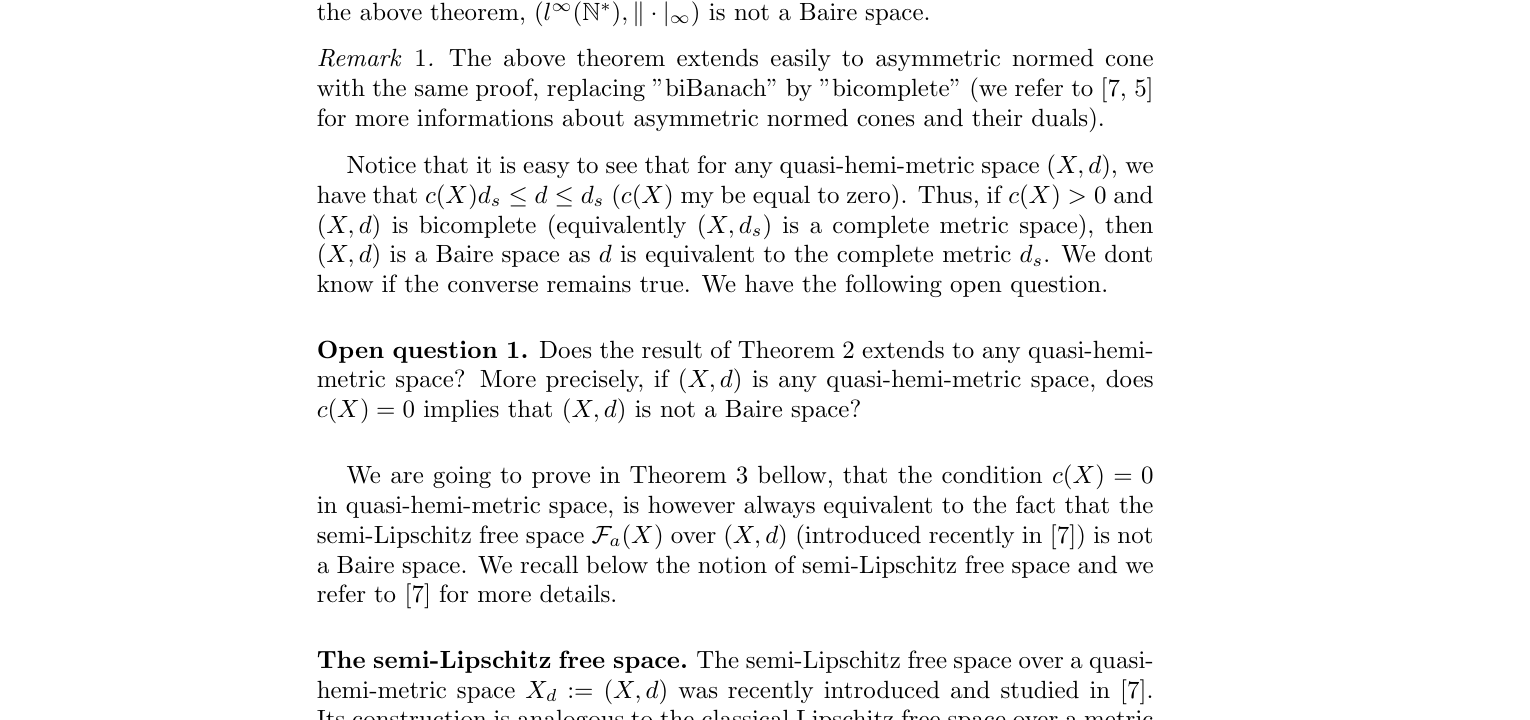
\includegraphics[width=\textwidth]{figures/open_question_1_crop.png}
\end{center}

On PDF page 8 it asks whether the semi-Lipschitz free space \(\Fa(X)\) of a
Baire quasi-hemi-metric space must itself be Baire. The source's Theorem 3,
shown in the same crop, states that \(c(X)=0\) if and only if \(\Fa(X)\) is not
Baire.

\begin{center}
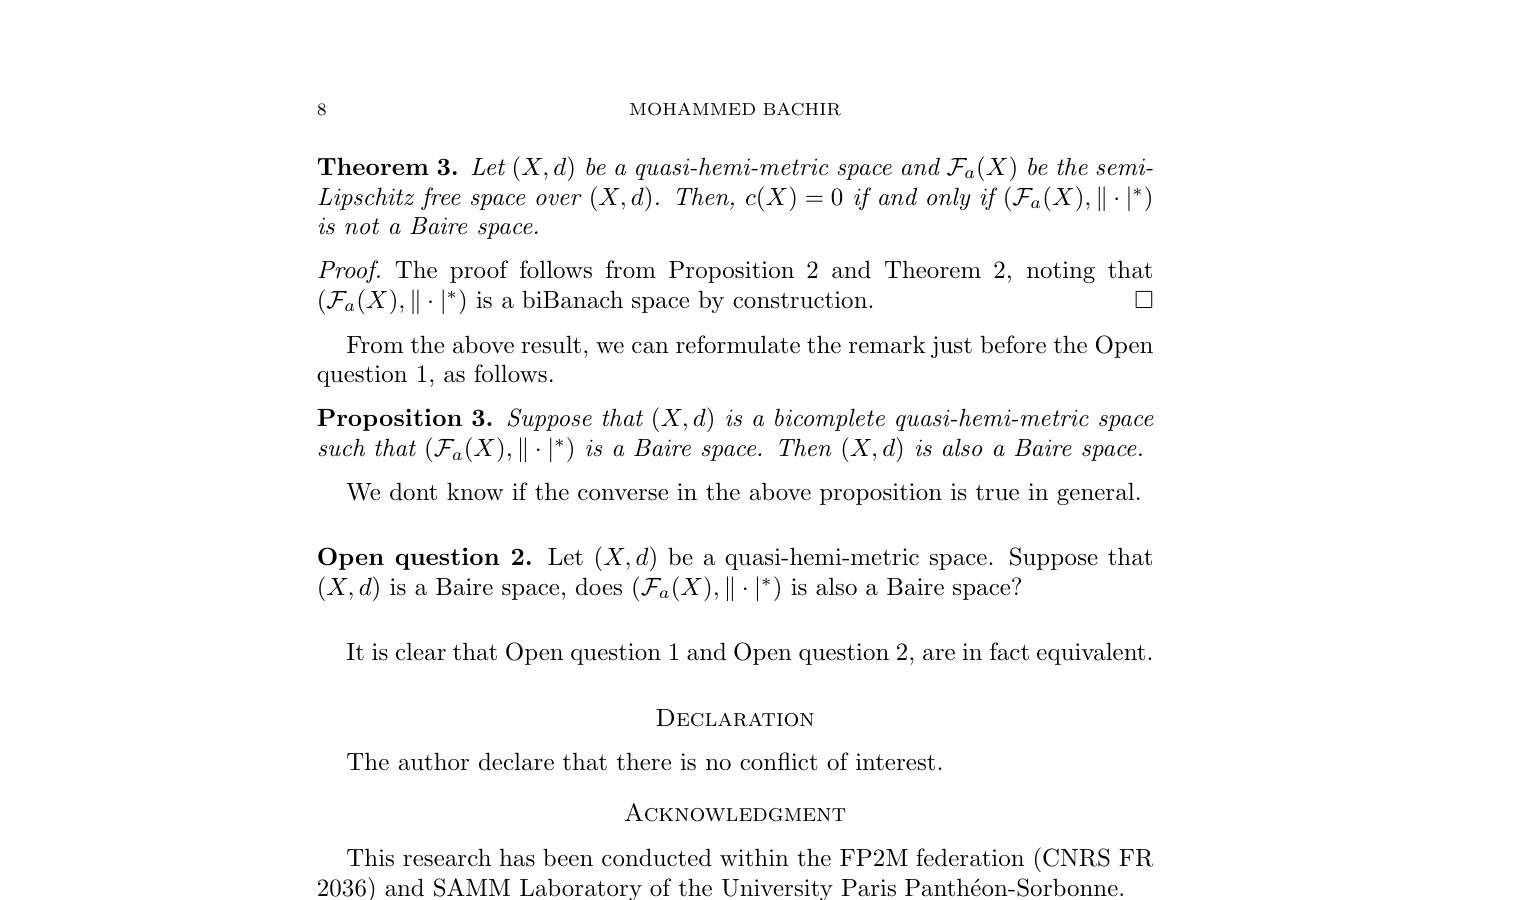
\includegraphics[width=\textwidth]{figures/open_question_2_crop.png}
\end{center}

\section*{Definitions}

For $a\in\R$, write $a_+=\max\{a,0\}$. A quasi-hemi-metric satisfies the
triangle inequality and separates distinct points after considering both
directions. A quasi-metric satisfies the stronger implication $d(x,y)=0$
only when $x=y$. Its forward balls are
\[
 B_d(x,r)=\{y:d(x,y)<r\}.
\]
The symmetrized metric is $d_s(x,y)=\max\{d(x,y),d(y,x)\}$, and the space is
bicomplete when $d_s$ is complete.

\section*{Idea of the Proof}

A directed potential $q_f(x,y)=(f(y)-f(x))_+$ always satisfies the triangle
inequality. We add the potentials $f(t)=t$ and $g(t)=e^{-t}$. The first
charges motion to the right, while the second charges motion to the left.
Both charges are locally comparable to Euclidean distance, so the forward
topology remains Euclidean. Far to the right, however, the leftward charge
across a unit interval is exponentially small while the rightward charge is
one. This destroys every global lower symmetry bound and forces $c(X)=0$.

\section*{Counterexample}

\begin{theorem}\label{thm:main}
Define $d:\R\times\R\to[0,\infty)$ by
\[
 d(x,y)=\pos{y-x}+\pos{e^{-y}-e^{-x}}.
\]
Then:
\begin{enumerate}
\item $d$ is a quasi-metric;
\item the topology generated by the forward $d$-balls is the usual
Euclidean topology on \(\R\), and hence \((\R,d)\) is a Baire space;
\item $c(\R,d)=0$;
\item the symmetrized metric is
\[
 d_s(x,y)=\max\{|x-y|,|e^{-x}-e^{-y}|\},
\]
and it is complete.
\end{enumerate}
Consequently, the implication proposed in Open Question 1 is false, even
among bicomplete quasi-metric spaces. Moreover, \(\Fa(\R,d)\) is not Baire,
so Open Question 2 is also false.
\end{theorem}

\begin{proof}
For an arbitrary real-valued function $f$ on a set, put
\[
 q_f(x,y)=\pos{f(y)-f(x)}.
\]
The elementary inequality \((u+v)_+\le u_++v_+\) gives
\[
 q_f(x,y)\le q_f(x,z)+q_f(z,y).
\]
Thus every $q_f$ satisfies the triangle inequality. Our function is the sum
of $q_f$ for $f(t)=t$ and $f(t)=e^{-t}$, so $d$ satisfies the triangle
inequality. Also $d(x,x)=0$. If $x<y$, then the first summand is $y-x>0$;
if $x>y$, then the second summand is $e^{-y}-e^{-x}>0$. Hence
$d(x,y)=0$ implies $x=y$, and $d$ is a quasi-metric.

For fixed $x$, the definition simplifies to
\[
 d(x,y)=
 \begin{cases}
 y-x,&y\ge x,\\
 e^{-y}-e^{-x},&y<x.
 \end{cases}\tag{1}
\]
The map $y\mapsto d(x,y)$ is Euclidean-continuous, so each forward ball
$B_d(x,r)$ is Euclidean-open. It follows that the $d$-topology is no finer
than the Euclidean topology.

Conversely, fix $x\in\R$ and \(\varepsilon>0\), and set
\[
 r=\min\left\{\varepsilon,
 e^{-(x-\varepsilon)}-e^{-x}\right\}>0.
\]
If $y\ge x$ and $d(x,y)<r$, then by (1),
$0\le y-x<r\le\varepsilon$. If $y<x$ but
$y\le x-\varepsilon$, then
\[
 d(x,y)=e^{-y}-e^{-x}
 \ge e^{-(x-\varepsilon)}-e^{-x}\ge r,
\]
a contradiction. Therefore
\[
 B_d(x,r)\subset(x-\varepsilon,x+\varepsilon).
\]
Every Euclidean neighborhood of $x$ thus contains a forward $d$-ball, so
the two topologies coincide. The real line with its Euclidean topology is a
Baire space; hence \((\R,d)\) is Baire.

Now take $x_n=n+1$ and $y_n=n$, for $n\ge0$. Formula (1) gives
\[
 d(y_n,x_n)=1,
 \qquad
 d(x_n,y_n)=e^{-n}-e^{-(n+1)}=(1-e^{-1})e^{-n}.
\]
The denominators $d(y_n,x_n)$ are positive, and therefore
\[
 0\le c(\R,d)
 \le \frac{d(x_n,y_n)}{d(y_n,x_n)}
 =(1-e^{-1})e^{-n}\longrightarrow0.
\]
Thus $c(\R,d)=0$.

If $x<y$, then $d(x,y)=y-x$ and
$d(y,x)=e^{-x}-e^{-y}$. Interchanging $x,y$ proves for all pairs that
\[
 d_s(x,y)=\max\{|x-y|,|e^{-x}-e^{-y}|\}.
\]
If \((x_k)\) is $d_s$-Cauchy, then it is Euclidean-Cauchy because
$|x_k-x_\ell|\le d_s(x_k,x_\ell)$. Hence $x_k\to x\in\R$. Continuity of
the exponential then gives
\[
 d_s(x_k,x)=
 \max\{|x_k-x|,|e^{-x_k}-e^{-x}|\}\longrightarrow0.
\]
Thus $d_s$ is complete and the example is bicomplete.

We have now produced a Baire quasi-metric space with $c(X)=0$, disproving
Open Question 1. Finally, Theorem 3 of the source paper \cite{Bachir} states
that $c(X)=0$ is equivalent to the asymmetric normed space \(\Fa(X)\) not
being Baire. Applying it here shows that \(\Fa(\R,d)\) is not Baire even though
\((\R,d)\) is Baire. This disproves Open Question 2.
\end{proof}

\begin{remark}
The example is deliberately outside the asymmetric normed setting of the
source's Theorem 2. The function $d$ is not translation invariant: the cost
of moving one unit to the left is $(1-e^{-1})e^{-x}$, which depends on the
base point $x$. Thus the counterexample does not contradict that theorem; it
shows exactly why its linear homogeneity cannot be dropped.
\end{remark}

\section*{Verification Notes}

The proof is elementary and self-contained apart from the source's Theorem 3,
which is used only to transfer the counterexample from Open Question 1 to Open
Question 2. The script \texttt{code/check\_counterexample.py} checks the
triangle inequality on a 13-point grid and 100,000 seeded random triples,
checks the displayed formula for $d_s$, and prints the symmetry ratios for
unit intervals. It completed with no violation. These finite tests are sanity
checks, not a substitute for the universal argument above.

\section*{Novelty and Limitations}

A bounded search on August 9, 2026 found no duplicate in the run indexes for
arXiv:2105.04862, quasi-hemi-metric Baire spaces, the symmetry index, or
semi-Lipschitz free spaces. Web searches used the exact title and DOI, the
phrases ``Open question 1'', ``$c(X)=0$ Baire quasi-metric'', ``index of
symmetry quasi-metric Baire'', and ``semi-Lipschitz free space Baire''. They
returned the source, bibliographic mirrors, and later background citations,
but no later claimed resolution. This is a bounded novelty check, not an
exhaustive citation or MathSciNet review.

The conclusion for Open Question 2 relies on Theorem 3 of the source paper.
The construction itself directly and independently settles Open Question 1.

\section*{Human Review Recommendation}

Accept as a likely valid counterexample after checking the orientation in the
definition of $c(X)$, the two topology inclusions, and the invocation of
source Theorem 3. There are no conditional lemmas or numerical dependencies.

\begin{thebibliography}{9}

\bibitem{Bachir}
M. Bachir,
\emph{Asymmetric Normed Baire Space},
Results in Mathematics \textbf{76} (2021), article 176;
arXiv:2105.04862v2,
\url{https://doi.org/10.1007/s00025-021-01483-6}.

\end{thebibliography}

\end{document}
